% **************************** Define Graphics Path **************************
\ifpdf
\graphicspath{{Chapter3/Figs/Raster/}{Chapter3/Figs/PDF/}{Chapter3/Figs/}}
\else
\graphicspath{{Chapter3/Figs/Vector/}{Chapter3/Figs/}}
\fi

\chapter{Thiết kế và Hiện thực}

\section{Thiết kế hệ thống}
\subsection{Kiến trúc mô hình hệ thống}
Lorem ipsum dolor sit amet, consectetur adipiscing elit, sed do eiusmod tempor incididunt ut labore et dolore magna aliqua. Ut enim ad minim veniam, quis nostrud exercitation ullamco laboris nisi ut aliquip ex ea commodo consequat. Duis aute irure dolor in reprehenderit in voluptate velit esse cillum dolore eu fugiat nulla pariatur. Excepteur sint occaecat cupidatat non proident, sunt in culpa qui officia deserunt mollit anim id est laborum
\subsection{Các ràng buộc của hệ thống}
Lorem ipsum dolor sit amet, consectetur adipiscing elit, sed do eiusmod tempor incididunt ut labore et dolore magna aliqua. Ut enim ad minim veniam, quis nostrud exercitation ullamco laboris nisi ut aliquip ex ea commodo consequat. Duis aute irure dolor in reprehenderit in voluptate velit esse cillum dolore eu fugiat nulla pariatur. Excepteur sint occaecat cupidatat non proident, sunt in culpa qui officia deserunt mollit anim id est laborum
\subsection{Mô hình ứng dụng trình bày dữ liệu}
Lorem ipsum dolor sit amet, consectetur adipiscing elit, sed do eiusmod tempor incididunt ut labore et dolore magna aliqua. Ut enim ad minim veniam, quis nostrud exercitation ullamco laboris nisi ut aliquip ex ea commodo consequat. Duis aute irure dolor in reprehenderit in voluptate velit esse cillum dolore eu fugiat nulla pariatur. Excepteur sint occaecat cupidatat non proident, sunt in culpa qui officia deserunt mollit anim id est laborum
\section{Hiện thực Node cảm biến}
\subsection{Các node cảm biến thu thập dữ liệu}
Lorem ipsum dolor sit amet, consectetur adipiscing elit, sed do eiusmod tempor incididunt ut labore et dolore magna aliqua. Ut enim ad minim veniam, quis nostrud exercitation ullamco laboris nisi ut aliquip ex ea commodo consequat. Duis aute irure dolor in reprehenderit in voluptate velit esse cillum dolore eu fugiat nulla pariatur. Excepteur sint occaecat cupidatat non proident, sunt in culpa qui officia deserunt mollit anim id est laborum
\subsection{Ứng dụng theo dõi dữ liệu và đánh giá}
Lorem ipsum dolor sit amet, consectetur adipiscing elit, sed do eiusmod tempor incididunt ut labore et dolore magna aliqua. Ut enim ad minim veniam, quis nostrud exercitation ullamco laboris nisi ut aliquip ex ea commodo consequat. Duis aute irure dolor in reprehenderit in voluptate velit esse cillum dolore eu fugiat nulla pariatur. Excepteur sint occaecat cupidatat non proident, sunt in culpa qui officia deserunt mollit anim id est laborum
\section{Hệ thống Server lưu trữ dữ liệu và cung cấp API}
Lorem ipsum dolor sit amet, consectetur adipiscing elit, sed do eiusmod tempor incididunt ut labore et dolore magna aliqua. Ut enim ad minim veniam, quis nostrud exercitation ullamco laboris nisi ut aliquip ex ea commodo consequat. Duis aute irure dolor in reprehenderit in voluptate velit esse cillum dolore eu fugiat nulla pariatur. Excepteur sint occaecat cupidatat non proident, sunt in culpa qui officia deserunt mollit anim id est laborum
\subsection{Cấu trúc tổ chức tập tin}
Lorem ipsum dolor sit amet, consectetur adipiscing elit, sed do eiusmod tempor incididunt ut labore et dolore magna aliqua. Ut enim ad minim veniam, quis nostrud exercitation ullamco laboris nisi ut aliquip ex ea commodo consequat. Duis aute irure dolor in reprehenderit in voluptate velit esse cillum dolore eu fugiat nulla pariatur. Excepteur sint occaecat cupidatat non proident, sunt in culpa qui officia deserunt mollit anim id est laborum
\subsection{Thiết kế API}
Lorem ipsum dolor sit amet, consectetur adipiscing elit, sed do eiusmod tempor incididunt ut labore et dolore magna aliqua. Ut enim ad minim veniam, quis nostrud exercitation ullamco laboris nisi ut aliquip ex ea commodo consequat. Duis aute irure dolor in reprehenderit in voluptate velit esse cillum dolore eu fugiat nulla pariatur. Excepteur sint occaecat cupidatat non proident, sunt in culpa qui officia deserunt mollit anim id est laborum

	\begin{lstlisting}[caption=My Javascript Example]
	Name.prototype = {
	methodName: function(params){
	var doubleQuoteString = "some text";
	var singleQuoteString = 'some more text';
	// this is a comment
	if(this.confirmed != null && typeof(this.confirmed) == Boolean && this.confirmed == true){
	document.createElement('h3');
	$('#system').append("This looks great");
	return false;
	} else {
	throw new Error;
	}
	}
	}
	\end{lstlisting}
\subsection{Xây dựng Web Server}
\subsection*{Chức năng}

\subsubsection*{Đối với người dùng:}
Hiện thị các node cảm biến đang hoạt động trên google map, cung cấp các thông tin liên quan đến node( vị trí địa lí, tình trạng hoạt động, biểu đồ theo thời gian thực của các dữ liệu mà node thu thập được), giao tiếp với người quản lý thông qua gmail.
\subsubsection*{Đối với người quản trị:}
Bao gồm các chức năng tương tự như người dùng và thêm việc quản lý chỉnh sửa thông tin của các node: thêm, xóa, cập nhật, thay đổi…

\subsection*{Biểu đồ High level Usecase }

\begin{center}
\begin{figure}[htp]
\centering    
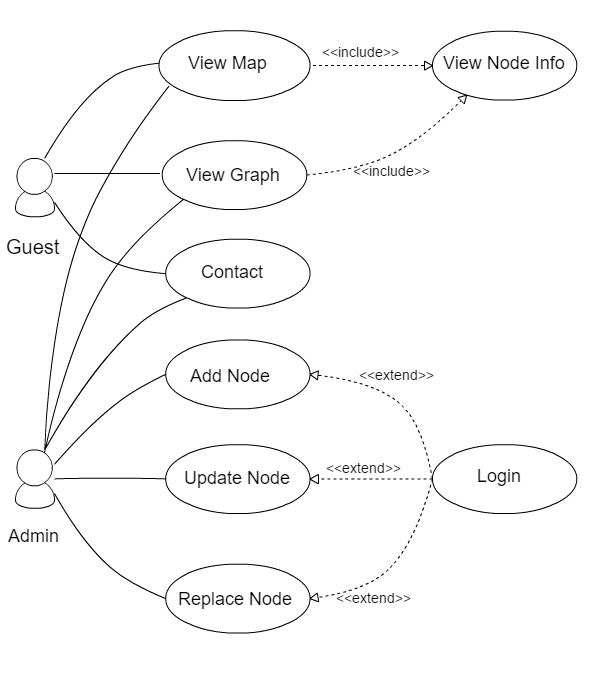
\includegraphics[width=0.7\textwidth]{usecase_diagram}
\caption[Biểu đồ High level Usecase]{Biểu đồ High level Usecase }
\label{fig:usecase_diagram}
\end{figure}
\end{center}

Mô tả giản đồ Usecase

\begin{table}[]
\centering
\caption{Bảng mô tả giản đồ Usecase của Web Server}
\label{my-label}
\begin{tabular}{|l|l|l|}
\hline
STT & Tên            & Miêu tả                                                                                            \\ \hline
1   & View map       & Người dùng thấy được các node đang chạy trên google maps                                           \\ \hline
2   & View Node Info & Thông tin tương ứng của Node( Lat, Lng, Phone)                                                     \\ \hline
3   & View Graph     & \begin{tabular}[c]{@{}l@{}}Đồ thị hoạt động của Node(các số liệu đo được theo\\ ngày)\end{tabular} \\ \hline
4   & Contact        & Phản hồi ý kiến người dùng qua Gmail                                                               \\ \hline
5   & Add Node       & Thêm mới Node vào hoạt động                                                                        \\ \hline
6   & Update Node    & Thay đổi thông tin của Node( Lat, Lng, Phone)                                                      \\ \hline
7   & Replace Node   & Thay đổi 1 Node xảy ra sự cố bằng 1 Node khác                                                      \\ \hline
\end{tabular}
\end{table}





\subsection*{Hiện thực giao diện}

Sử dụng framework express của Nodejs và HTML để xây dựng frontend


\subsubsection*{Giao diện chính của Web Server}
Phần này chứa các nút menu chức năng cùng với google map để theo dõi vị trí hoạt động của các cảm biến.
\begin{center}
\begin{figure}[htp]
\centering    
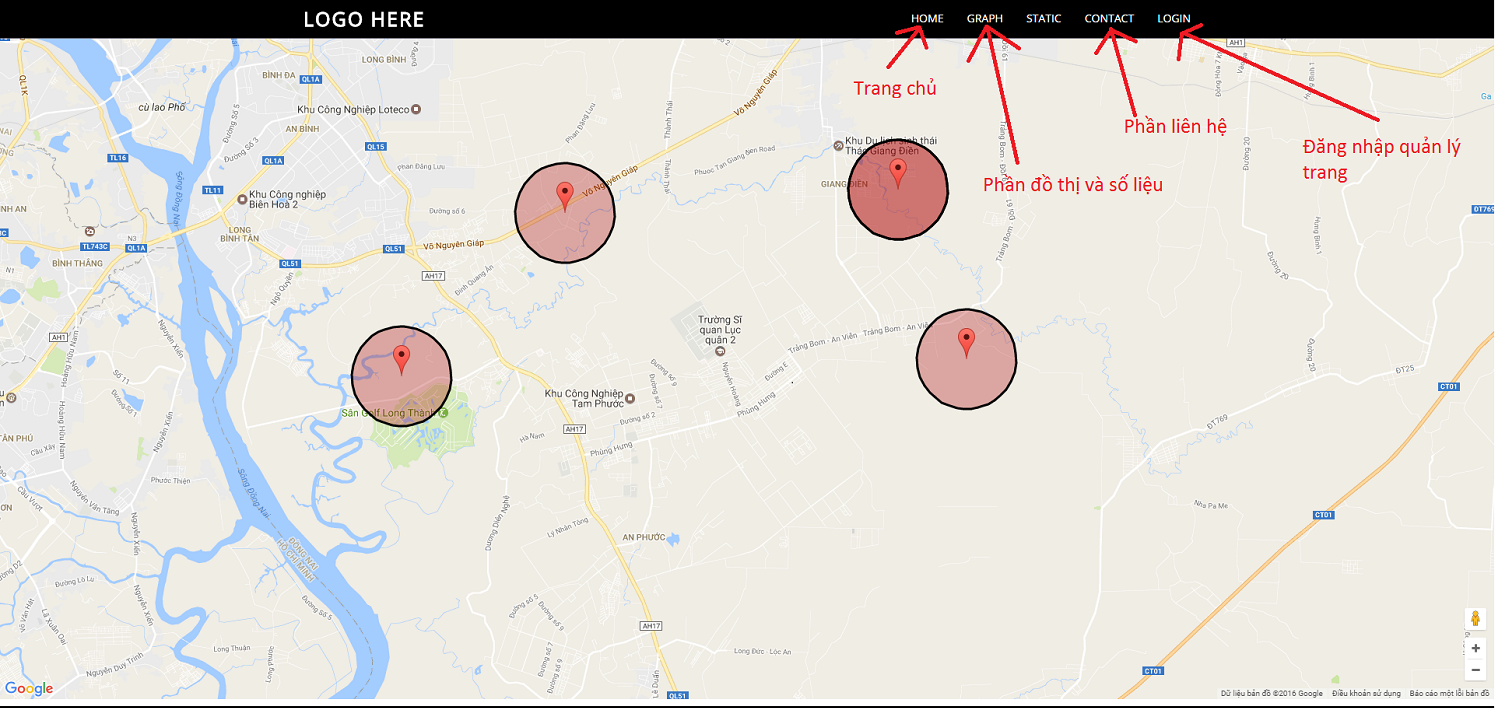
\includegraphics[width=1\textwidth]{webserver}
\caption[Giao diện chính của Web Server]{Giao diện chính của Web Server}
\label{fig:webserver}
\end{figure}
\end{center}

\subsubsection*{Giao diện đồ thị dữ liệu}
Là nơi hiện thị biểu đồ của các thông số cũng như thông tin tương ứng của các cảm biến.
\begin{center}
\begin{figure}[htp]
\centering    
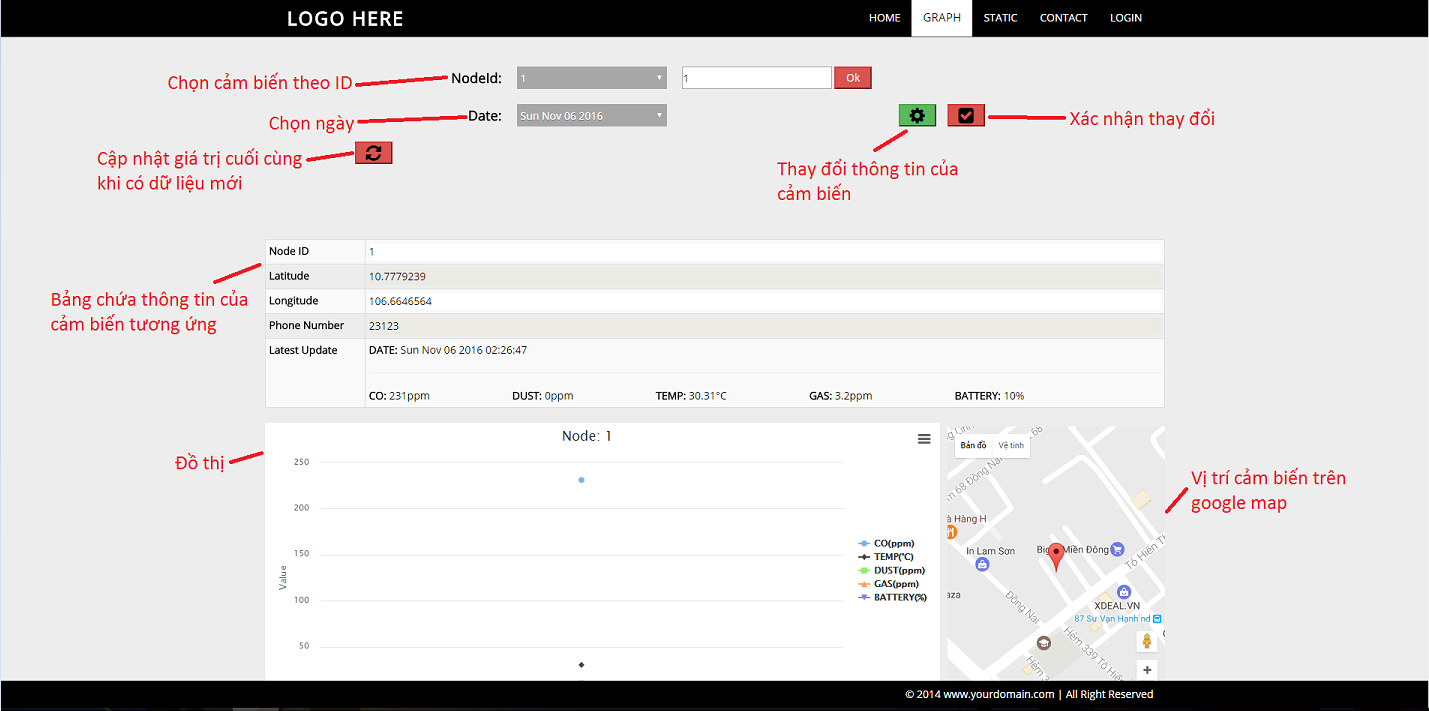
\includegraphics[width=1\textwidth]{web_graph}
\caption[Giao diện đồ thị dữ liệu]{Giao diện đồ thị dữ liệu}
\label{fig:web_graph}
\end{figure}
\end{center}



\subsubsection*{Giao diện nhận feedback từ người dùng qua email}
Tương tác giữa người dùng với người quản lý server. Nội dung được gửi thông qua gmail.
\begin{center}
\begin{figure}[htp]
\centering    
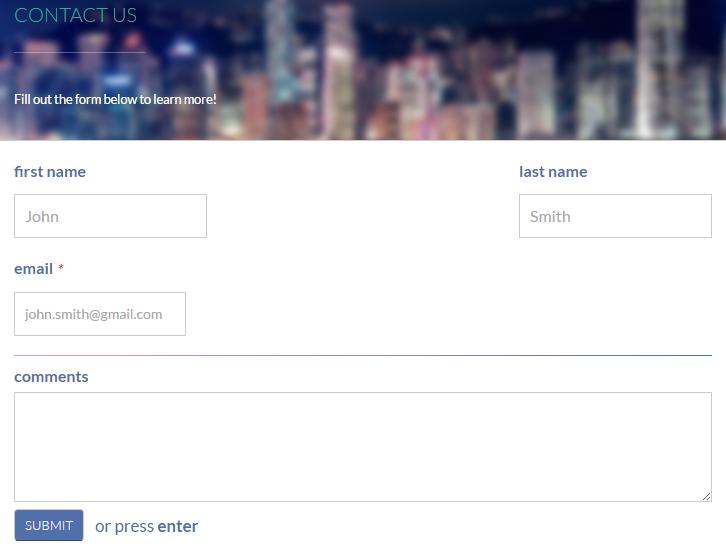
\includegraphics[width=1\textwidth]{web_email}
\caption[Giao diện nhận feedback người dùng]{Giao diện nhận feedback người dùng}
\label{fig:web_email}
\end{figure}
\end{center}

\subsubsection*{Giao diện dành cho người quản lý}
Khu vực này dành cho người quản lý truy cập nhầm mục đích chỉnh sửa, thay thế các node cảm biến.
\begin{center}
\begin{figure}[htp]
\centering    
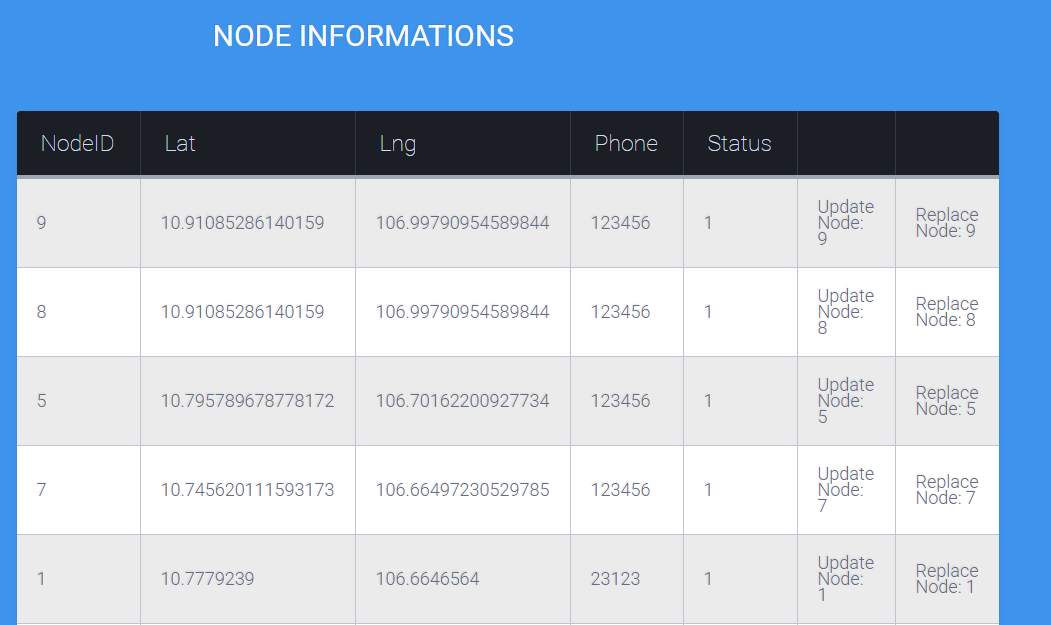
\includegraphics[width=1\textwidth]{web_nodeinfo}
\caption[Giao diện quản lý các node cảm biến]{Giao diện quản lý các node cảm biến}
\label{fig:web_nodeinfo}
\end{figure}
\end{center}





\section{Ứng dụng thiết bị di động}

\subsection{Chức năng}
Hiện thị thông tin các node cảm biến đang hoạt động qua màn hình chính, và biểu đồ dữ liệu của từng node cảm biến theo từng ngày, thêm sự kết nối với web browser tạo sự thuận tiện cho việc theo dõi, hiện thị đồ thị (2 kiểu đồ thị là line chart và bar chart).

\subsection{Biểu đồ High level Usecase}

\begin{center}
\begin{figure}[htp]
\centering    
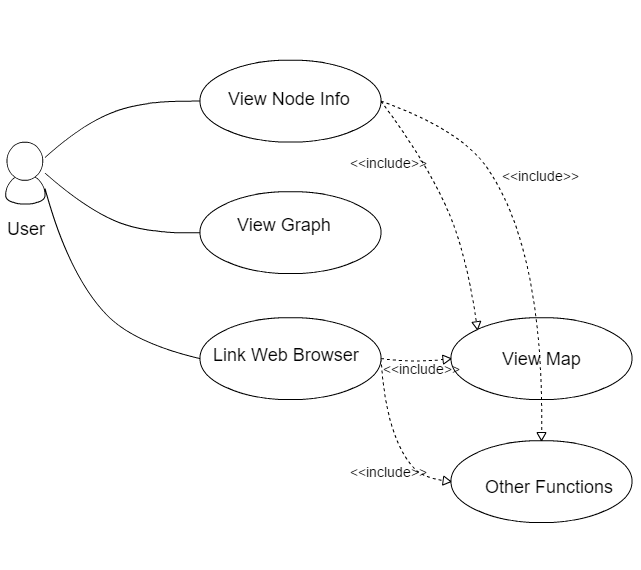
\includegraphics[width=1\textwidth]{app_usecase}
\caption[Giản đồ High level Usecase của ứng dụng di động]{Giản đồ High level Usecase của ứng dụng di động}
\label{fig:app_usecase}
\end{figure}
\end{center}



Mô tả Usecase

\begin{table}[]
\centering
\caption{Bảng mô tả giản đồ Usecase của ứng dụng di động}
\label{table:usecase_mobile}
\begin{tabular}{|l|l|l|}
\hline
STT & Tên Use-case     & Mô tả                                                            \\ \hline
1   & View Node Info   & Thông tin của Node( Lat, lng, Phone, ID)                         \\ \hline
2   & View Graph       & 2 dạng đồ thị theo ngày (line chart, bar chart của các thông số) \\ \hline
3   & Link web browser & Liên kết tới web browser                                         \\ \hline
4   & View Map         & Hiện thị Google Map và vị trí các Node                           \\ \hline
5   & Other Functions  & Các chức năng của web browser                                    \\ \hline
\end{tabular}
\end{table}


\subsection{Hiện thực giao diện và chức năng}
\subsubsection*{Giao diện chính ứng dụng di động}
Tại giao diện chính của ứng dụng di động người dùng có thể xem được danh sách thông tin chi tiết của các node cảm biến có trong hệ thống.
\begin{center}
\begin{figure}[htp]
\centering    
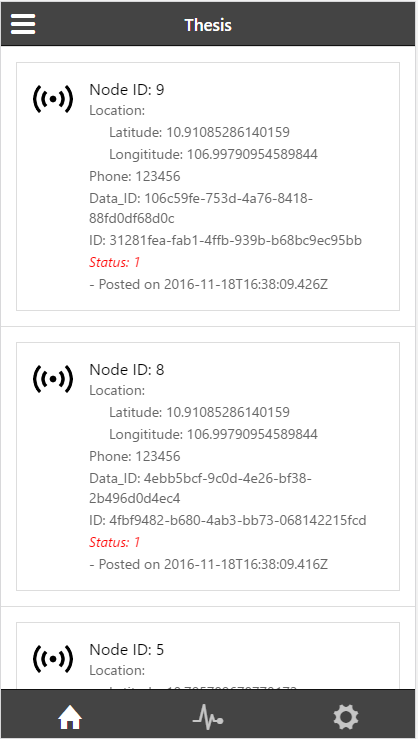
\includegraphics[width=0.4\textwidth]{app_main}
\caption[Giao diện chính ứng dụng di động]{Giao diện chính ứng dụng di động}
\label{fig:app_main}
\end{figure}
\end{center}


\subsubsection*{Giao diện xem dữ liệu trên ứng dụng di động}
Giao diện này cho phép người dùng theo dõi được dữ liệu của từng node cảm biến theo 2 loại biểu đồ như Hình \ref{fig:app_graph} thể hiện.
\begin{center}
\begin{figure}[htp]
\centering    
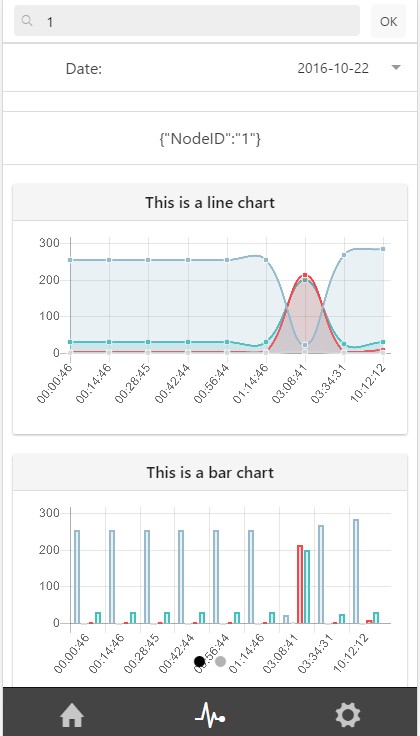
\includegraphics[width=0.4\textwidth]{app_graph}
\caption[Giao diện xem dữ liệu trên ứng dụng di động]{Giao diện xem dữ liệu trên ứng dụng di động}
\label{fig:app_graph}
\end{figure}
\end{center}


